% paper/sections/12u6_split_ppe_dc_hfe.tex
%
% U6: DC/HFE primitives for phase-separated PPE — Tier IV
% ═══════════════════════════════════════════════════════════════════════════════
\subsubsection{U6：分相 PPE+HFE へ渡す DC/HFE primitive [Tier IV]}
\label{sec:U6_split_ppe_dc_hfe}
\label{sec:varrho_ppe_limitation}%   forward-pointer alias from §9 / §15

\paragraph{検証対象．}
第~\ref{sec:ppe_solve}章および第~\ref{sec:algorithm}章の標準圧力経路は，
\textbf{pressure-jump 分相 PPE + HFE + DC}である．
変密度一括 smoothed-Heaviside PPE は低密度比の対照・経路選択診断に限り，
高密度比の保証対象 primitive ではない．したがって本 U6 は，一括 PPE 高密度比 sweep を
成果サブテストとして数えず，分相 PPE+HFE に渡す二つの前提 primitive：
(i) defect--correction（DC；§\ref{sec:dc_pure_fccd_convergence}）の
$\omega$--緩和 guard と，
(ii) Hermite Field Extension（HFE；§\ref{sec:hfe}）による界面越し場延長の
\textbf{単体精度}を確認する．

\paragraph{設定．}
\begin{description}\setlength{\itemsep}{0pt}
  \item[U6-a] DC $\omega$--緩和 guard．$N=64$ 円界面 $R=0.25$，
        $\rho_l \in \{1, 100, 1000\}$，relaxation $\omega \in \{0.2,0.3,0.5,0.7,0.9\}$，
        $k_{\mathrm{DC}} \in \{2,3\}$．低密度比では clean であること，高密度比では一括 PPE を
        保証対象 primitive と見なせないことを route guard として記録する．
  \item[U6-b] HFE 単独：1D MMS（外挿ステンシル単体精度），
        2D MMS（$\rho^{-1}\bnabla p$ の界面跨ぎ精度の \textbf{max} と \textbf{med}）．
\end{description}

\paragraph{結果．}

\begin{table}[!ht]
\caption{U6-a：DC \texorpdfstring{$\omega$}{omega}--緩和 guard}
\label{tab:U6_dc_omega}
\PaperCaptionNote{$N=64$，円界面 $R=0.25$．$\rho_l = 1$ は低密度比対照として clean．$\rho_l \ge 100$ では一括 PPE 係数ジャンプが残るため DC 残差が route guard にかかり，高密度比保証対象 primitive から除外される．$\omega$ 増大で残差は改善するが，$\rho_l = 1000$, $\omega = 0.9$, $k=3$ の例外的な許容床到達は経路受理条件ではなく，分相 PPE+HFE へ切り替える判断を変えない．括弧内は \emph{converged} を示す．}
\centering\small
\begin{tabular}{r c c c c c}
\toprule
 & \multicolumn{2}{c}{$k_{\mathrm{DC}}=2$} & \multicolumn{2}{c}{$k_{\mathrm{DC}}=3$} & $\rho_l=1$ \\
\cmidrule(lr){2-3}\cmidrule(lr){4-5}\cmidrule(lr){6-6}
$\omega$ & $\rho_l\!=\!100$ & $\rho_l\!=\!1000$ & $\rho_l\!=\!100$ & $\rho_l\!=\!1000$ & all $k$ \\
\midrule
$0.2$ & $8.69\!\times\!10^{-3}$ & $5.57\!\times\!10^{-4}$ & $6.95\!\times\!10^{-3}$ & $4.46\!\times\!10^{-4}$ & $5.19\!\times\!10^{-5}$ \\
$0.3$ & $7.60\!\times\!10^{-3}$ & $4.88\!\times\!10^{-4}$ & $5.32\!\times\!10^{-3}$ & $3.42\!\times\!10^{-4}$ & $5.19\!\times\!10^{-5}$ \\
$0.5$ & $5.43\!\times\!10^{-3}$ & $3.49\!\times\!10^{-4}$ & $2.71\!\times\!10^{-3}$ & $1.74\!\times\!10^{-4}$ & $5.19\!\times\!10^{-5}$ \\
$0.7$ & $3.26\!\times\!10^{-3}$ & $2.09\!\times\!10^{-4}$ & $9.77\!\times\!10^{-4}$ & $6.28\!\times\!10^{-5}$ & $5.19\!\times\!10^{-5}$ \\
$0.9$ & $1.09\!\times\!10^{-3}$ & $7.00\!\times\!10^{-5}$ & $1.09\!\times\!10^{-4}$ & $\mathbf{7.00\!\times\!10^{-6}}^{\dagger}$ & $5.19\!\times\!10^{-5}$ \\
\bottomrule
\end{tabular}
\\[2pt]
{\footnotesize $\dagger$: $\rho_l=1000$, $\omega=0.9$, $k=3$ は唯一 stall せず converge．
$\omega \ge 0.5$ で残差が単調減少し，$\omega=0.9$ で $k=2 \to k=3$ により 10$\times$ 改善．}
\end{table}

\begin{table}[!ht]
\caption{U6-b：HFE 単独 MMS（外挿ステンシル）}
\label{tab:U6_hfe}
\PaperCaptionNote{\textbf{1D} は設計通り 6 次近傍（slope $\approx 5.91$, $N=32\!\to\!256$）．\textbf{2D} band は完全テンソル修正後に低次化が消え，$N=64$ 以降で $10^{-7}$ から丸め床近傍まで急減する．slope 行は $N=32$ の closest-point 前漸近と細格子側の丸め床を含む \textbf{2 点 endpoint slope}（$N\!=\!32 \to 256$ 端点；多点 log--log fit ではない）であり，形式次数は $\Ord{h^6}$ と読む．}
\centering\small
\begin{tabular}{r r r r r}
\toprule
$N$ & $h$ & $\|e^{1\mathrm{D}}\|_\infty$ & $\|e^{2\mathrm{D}}_{\max}\|$ & $\|e^{2\mathrm{D}}_{\mathrm{med}}\|$ \\
\midrule
$32$  & $0.0313$ & $9.19\times 10^{-8}$ & $1.02\times 10^{-3}$ & $3.47\times 10^{-7}$ \\
$64$  & $0.0156$ & $1.62\times 10^{-9}$ & $4.01\times 10^{-7}$ & $2.09\times 10^{-10}$ \\
$128$ & $0.0078$ & $2.68\times 10^{-11}$ & $1.22\times 10^{-11}$ & $7.75\times 10^{-13}$ \\
$256$ & $0.0039$ & $4.22\times 10^{-13}$ & $5.80\times 10^{-14}$ & $4.55\times 10^{-15}$ \\
\midrule
\multicolumn{2}{r}{effective slope ($N\!=\!32\!\to\!256$)} & $\mathbf{5.91}$ & $\mathbf{11.35}$ & $\mathbf{8.72}$ \\
\bottomrule
\end{tabular}
\end{table}

\begin{figure}[!ht]
\centering
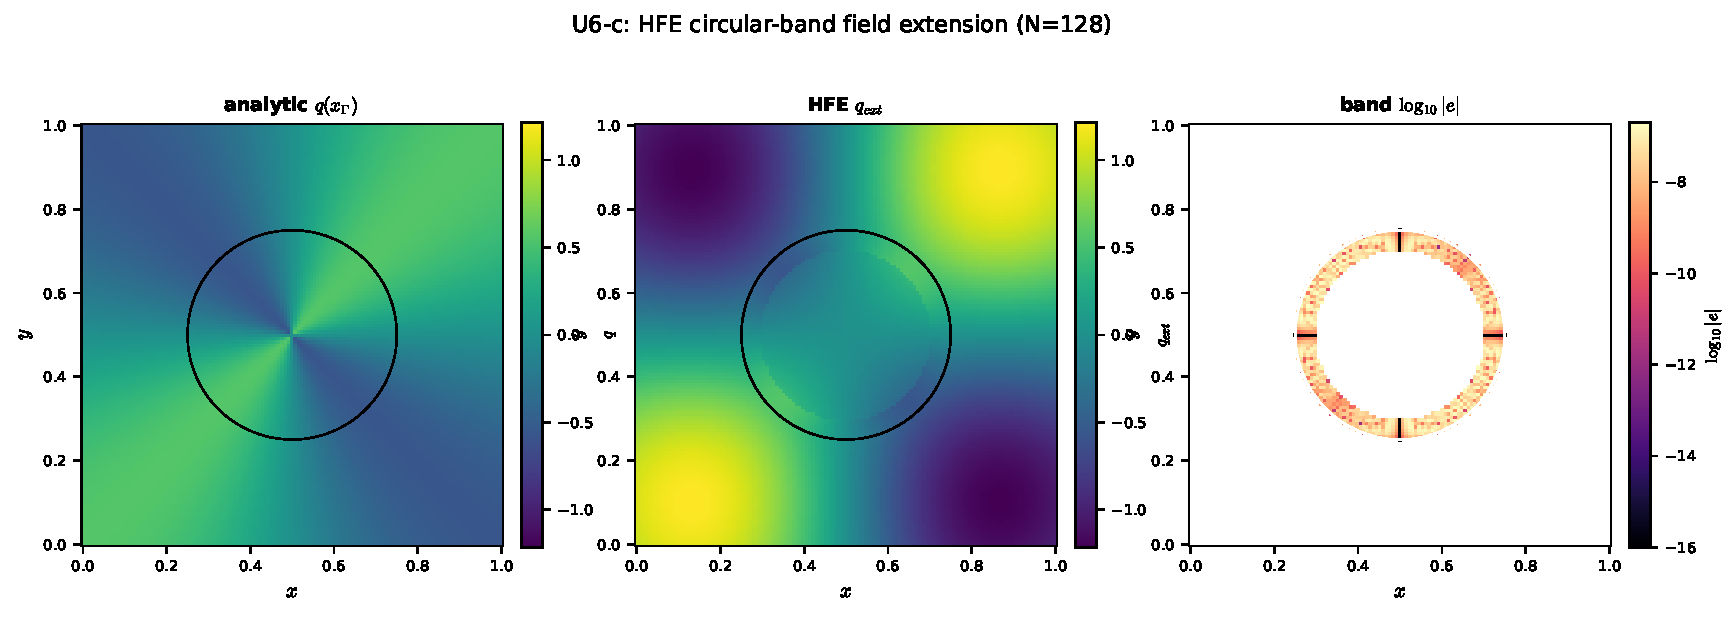
\includegraphics[width=0.92\linewidth]{figures/ch12_u6_hfe_2d_field}
\caption{U6-b：HFE 2D circular-band 場延長マップ (\texorpdfstring{$N=128$}{N=128})}
\label{fig:ch12_u6_hfe_field}
\PaperCaptionNote{左：円形界面 $\Gamma$ 上の最近接点解析値 $q(\bx_\Gamma)$， 中央：Hermite Field Extension による延長場 $q_{\mathrm{ext}}$， 右：target band ($\phi \ge 0$, $|\phi|\le 6h$) 内の $\log_{10}|q_{\mathrm{ext}}-q(\bx_\Gamma)|$． 等高線は $\phi=0$ であり，\autoref{sec:hfe} の最近接点 Hermite 延長を 2D 円形界面上で直接可視化したものである．}
\end{figure}

\paragraph{判定と次章への接続．}
\begin{itemize}\setlength{\itemsep}{0pt}
  \item U6-a DC $\omega$--緩和 guard：$\rho_l = 1$ は低密度比対照として clean．
        $\rho_l \ge 100$ では一括 PPE の係数ジャンプが残り，$\omega$ 増大で残差が改善しても
        高密度比の受理経路にはしない．例外的な $\rho_l = 1000$, $\omega=0.9$,
        $k_{\mathrm{DC}}=3$ の許容床到達は route guard を解除する根拠ではなく，
        §\ref{sec:split_ppe_framework} の分相 PPE+HFE 経路選択を支持する負対照である．\checkmark
  \item U6-b HFE：1D stencil は設計 6 次を完全達成．2D circular band も
        完全テンソル混合微分を用いることで低次化が消える．
        $N=32$ の max は closest-point 幾何の前漸近を含むが，
        $N=64$ 以降は丸め床近傍まで急減し，§\ref{sec:hfe} の
        $\Ord{h^6}$ 設計と一致する．\checkmark
\end{itemize}
検証対応：
DC 反復収束は分相 PPE+HFE 経路へ入る前の緩和 guard として測定する．
高密度比・二相結合系の統合検証は，一括 PPE ではなく V6/V7/V9 の
FCCD, HFE, 圧力ジャンプ付き分相 PPE/DC, 毛管成分の圧力勾配射影,
射影後面速度閉包，アフィン圧力履歴面加速度を含む
圧力ジャンプ・毛管射影結合系で行う．
式~\eqref{eq:hfe_upwind_minus}（HFE 拡張公式）については，1D/2D の外挿誤差を測定する．

\FloatBarrier
